%-------------------------------------------------------------------------------
\chapter{Mély tanuló alkalmazások fejlesztése}
%-------------------------------------------------------------------------------
A mély tanulás, konkrétabban a mesterséges neurális hálózatok gyors fejlődősét és részben népszerűségét a hozzá készített programozási keretrendszereknek köszönheti, melyek java szabad hozzáférésű. Ezek a keretrendszerek arra hivatottak, hogy támogassák a neurális hálózatok fejlesztését új programozási módszertant adva. Már létező programozási nyelvekre épülnek, leginkább python-ra. Ezekben a keretrendszerekben egyszerűen implementálhatunk neurális hálózatokat úgy, hogy egyfajta nyelvi eszközkészletet adnak neurális hálózatok definiálására.

\section{TensorFlow}

%TODO Nincs Befejezve
\section{Keras}
A Keras egy python nyelven írt programkönyvtár, vagy ahogy önmagát hívja ''magas szintű neurális hálózat API''\cite{web:Keras}. Fejlesztésébe François Chollet kezdett bele. Érdekessége, hogy más olyan keretrendszerekkel együttesen használható, amelyek a Keras-hoz hasonlóan magas absztrakciós szinten biztosítják a hálózatok implementálását, mint például a TensorFlow.
%A Keras-ról szerzett tudásom javát Chollet könyvéből és a keretrendszer dokumentációjából szereztem.\cite{Chollet}\cite{web:Keras}.
Chollet könyve részletesen bemutatja a keretrendszer használatát, továbbá nyíltan hozzáférhető annak dokumentációja is.\cite{chollet}\cite{web:Keras}
\begin{figure}[h]
	\centering
	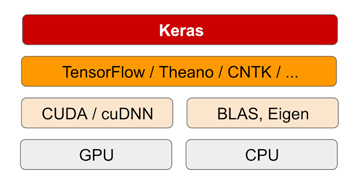
\includegraphics[width=0.5\linewidth]{fig/keras_software_stack}
	\caption{Keras szoftver rendszer\protect\footnotemark}
	\label{fig:kerassoftwarestack}
\end{figure}
\footnotetext{Forrás:\protect\cite{chollet}}

\subsection{Neurális hálózat definiálása}
Keras-ban egy neurális hálózatot \emph{model}-nek hívunk (gyakran máshol is így neveznek egy konkrét neurális hálózatot). Egy \emph{model} létrehozásához a \verb|Keras.models| modulban definiált metódusokkal lehetséges. A keretrendszerben az adatokat tenzorokként kell reprezentálnunk, ezért érdemes a \emph{numpy}\footnote{lásd:\url{https://numpy.org/}} nevű python csomaggal együtt használni. A keretrendszer tetszőleges alakú tenzorokat képes kezelni, tehát nincs megkötés arra vonatkozóan, hogy egy réteg bemenete vektor, mátrix vagy kiterjedtebb struktúrában -- magasabb dimenziójú tenzorban -- szerepeljen. A következő kódokban szeretném szemléltetni a Keras használatának módját.

A \ref{lst:defLayers} kód egy két rétegből álló neurális hálózat definiálását mutatja be.
\begin{minipage}{\textwidth}
\begin{lstlisting}[language=Python, caption=Neurális hálózat rétegeinek definiálása]
from keras import models
from keras import layers

network = models.Sequential()
network.add(layers.Dense(15, activation='relu', input_shape=(784,)))
network.add(layers.Dense(10, activation='softmax'))
\end{lstlisting}\label{lst:defLayers}
\end{minipage}
Ezen lista 4. sorában inicializáljuk a hálózatot, az utána következő sorokban új neuron rétegeket adunk a hálózathoz.Keras-ban különböző előre definiált rétegkapcsolatok vannak. Itt a \verb|layers.Dense| osztály egy sűrűn kapcsolt réteget implementál. %TODO sürün kapcsolt réteg definíciója
A réteg bemenetként $28 *28 = 784$ elemű vektorokból álló mátrixot tud fogadni, másik dimenziója nem meghatározott. Ez a kötegelt adatfeldolgozás szempontjából fontos, tehát a bemeneti vektorok folyamát egyik dimenziójában nem meghatározott méretű tenzorral definiáljuk. A réteg kimenete egy 32 dimenziós vektor. A következő rétegnél nem adtuk meg a bemenet méretét, a keretrendszerben ez implicit módon rendelődik a réteghez. 

Mindkét réteghez tartozik egy \emph{activation} paraméter, mely string típus kell legyen, és a réteg neuronjaihoz tartozó aktivációs függvényt adja meg. A példában a \verb|'relu'| és \verb|'softmax'| string a \ref{sec:fuggvenyek-algoritmusok} fejezet \eqref{eq:relu} és \eqref{eq:softmax} függvényére utal, azaz ezen bemeneti paraméterek esetén olyan \verb|Dense| objektum jön létre, mely ilyen aktivációs függvényekkel rendelkező neuron réteget valósít meg.

A \verb|Keras.layers| modulban A \verb|Dense| osztályon kívül implementálva vannak konvolúciós, összefésülő, zaj, stb. rétegek, melyek a fenti módon tetszés szerint egymásra szervezhetőek a keretrendszerben, így szinte tetszőleges hálózat alakítható ki.

\subsection{Hálózat betanítása és betanított hálózat futtatása}
\label{subsect:inference}
A megalkotott hálózatot a \verb|network| objektum definiálja. Hogy tanítható legyen el kell látni egy optimizálóval és egy veszteségfüggvénnyel, melyek együtt adják a hálózatot betanító algoritmust. A \verb|compile()| metódus ,,összerakja'' a neurális hálózatot a betanítóval, a \verb|fit()| pedig elvégzi a tanítást, és \emph{epoch}-ok számának megfelelő méretű tömböket tartalmazó objektum referenciájával tér vissza, mely tömbökben össze vannak gyűjtve a veszteségfüggvény értékei és a felhasználói metrikák eposzonként. 
\begin{minipage}{\textwidth}
\begin{lstlisting}[language=Python,caption=Hálózat betanítása]
network.compile(optimizer = 'sgd',
loss = 'mean_squared_error',
metrics = ['acc'])

history = network.fit(train_datas,
						train_labels,
						epochs=20,
						batch_size=512)
\end{lstlisting}\label{lst:fitNetwork}
\end{minipage}

A \verb|train_datas| és \verb|train_labels| a tanítókészletet alkotó minták és azok címkéi, a várt kimeneti értékek. Ezek elemszáma kötelezően meg kell egyezzen. A \emph{batch\_size} paraméterrel, ami az egy \emph{epoch}-ban egyszerre feldolgozandó adatokat jelenti. A betanítás végén a \verb|network| egy \emph{betanított}, a célfeladat megoldására felhasználható neurális hálózat lesz. Alkalmazásához a \verb|predict()|metódus használatos,mely a paraméterként megadott bemeneti adatokhoz tartozó predikciókkal tér vissza.
\begin{minipage}{\textwidth}
\begin{lstlisting}[language=Python, caption=Az eszközre töltött hálózat futtatása az adatokon]
	result = network.predict(datas)
\end{lstlisting}
\end{minipage}

\subsection{Hatékonyságvizsgálat}

A tanítás felügyeletére a tanításhoz rendelkezésre álló adatok egy részét külön kell választanunk a tanítókészlettől. Ez a készlet lesz a validálási készletünk, mellyel minden tanítási ciklus végén leellenőrizzük, hogy hogyan teljesít a hálózat olyan adaton, amit még ,,nem látott''. A validálást Keras-ban megtehetjük a tanítással egy lépésben, a \verb|fit()| algoritmussal, ha a \verb|validation_data| opcionális paraméterének megadunk egy \verb|(data, label)| \verb|tuple| típusú változót. Ekkor a metódus olyan referenciával tér vissza (\ref{lst:fitNetwork}~kódrészletben ez a \verb|history|), melyen keresztül a tanítási és validálás statisztikák is beolvashatóak. A \ref{subsect:inference}~szakaszban említett metrikák a validálási folyamathoz is rögzítve lesznek. 
\begin{figure}[H]
	\centering
	\begin{subfigure}{0.45\textwidth}
		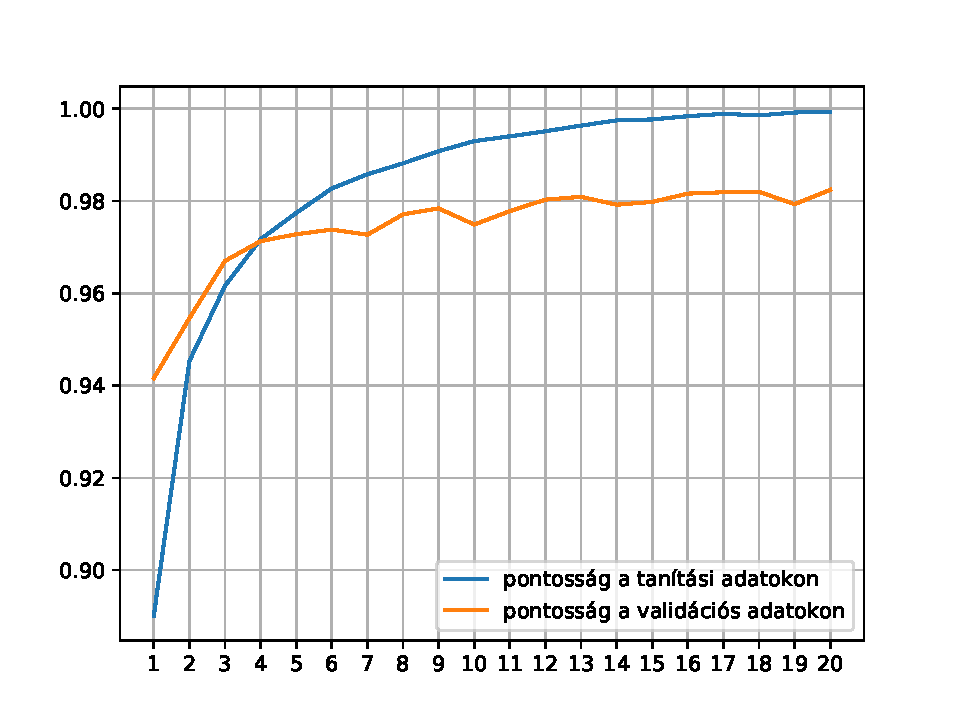
\includegraphics[width=\textwidth]{fig/accuracy.pdf}
		\label{fig:plotacc}
	\end{subfigure}
	\quad
	\begin{subfigure}{0.45\textwidth}
		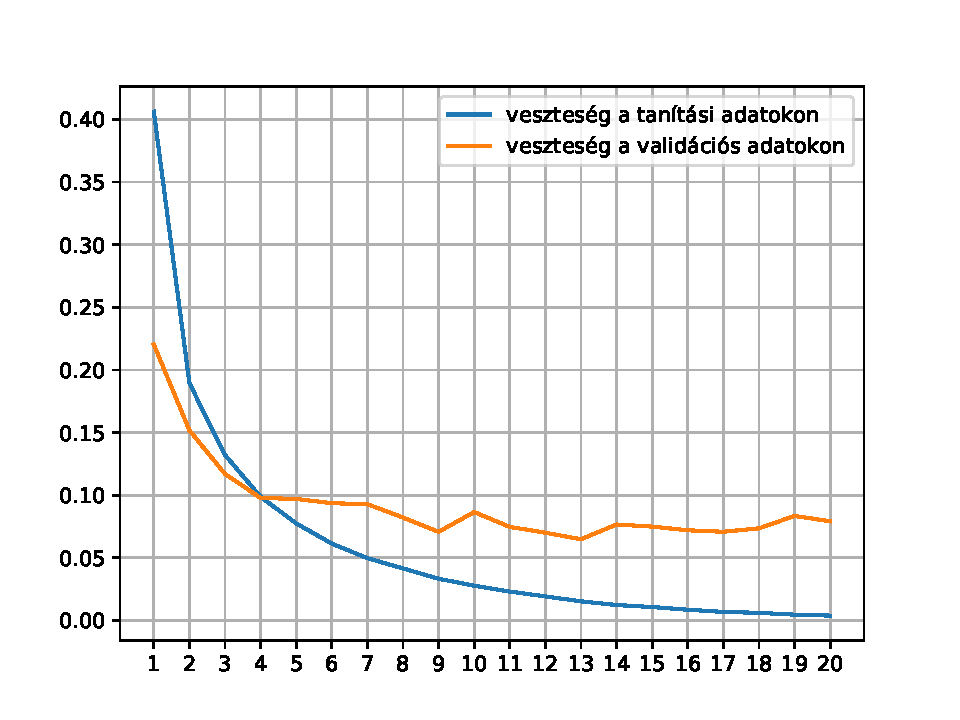
\includegraphics[width=\textwidth]{fig/loss.pdf}
		\label{fig:plotloss}
	\end{subfigure}
	\caption{Példa kimutatás a Keras által gyűjtött statisztikákról}
\end{figure}
%TODO Nincs Befejezve